% !TEX root = trackjet_intnote.tex

\subsection{Data samples}
%\label{sec:data}

This analysis used the original processing of \pp\ (reconstruction tag 7744) and \PbPb\ (reconstruction tag 7874) collisions at \sqrtsnn~=~5.02~TeV recorded in 2015 with a total integrated luminosity of 25 pb$^{-1}$ and 0.49~nb$^{-1}$ respectively. The run numbers for each set are given below:
\begin{itemize}
\item 2015 \pp\ data: 286282, 286361, 286364, 286367, 286411, 286474
\item 2015 \PbPb\ data: 286711, 286717, 286748, 286767, 286834, 286854, 286908, 286990, 287038, 287044, 287068, 287222, 287224, 287259, 287270, 287281, 287321, 287330, 287334, 287378, 287380, 287382, 287560, 287594, 287632, 287706, 287728, 287827, 287843, 287866, 287924, 287931
\end{itemize}


%\begin{itemize}
%   \item
%286711,  287068,  287560,
%286717,  287222,  287594,
%286748,  287224,  287632,
%286767,  287259,  287706,
%286834,  287270,  287728,
%286854,  287281,  287827,
%286908,  287321,  287843,
%286967,  287330,  287866,
%286990,  287334, 287924,
%286995,  287378,  287931,
%287038,  287380,
%287044,  287382
%\end{itemize}
Various hard probe triggers (high-\pT\ jets, muons, electrons, and photons) are group into a Hard Probe (HP) stream and Main stream in \PbPb\ and \pp\ data taking periods respectively. The \pp\ data samples from the Main stream used in this analysis are listed in Table~\ref{tab:events}. For the analysis of the \pbpb\ data the officially produced HION7 derivation samples from the Hard Probe stream are used. The list of datasets together with detailed description of HION7 derivation setup can be found in Ref.~\cite{HIdataderviation}. Additionally to the jet triggered data sample, \PbPb\ collisions recorded by Minimum-Bias (MB) triggers grouped in to MB stream are utilized in this analysis. The following MB data sets are used: \texttt{data15\_hi.0028*.physics\_MinBias.merge.AOD.r7874\_p2580}.



\begin{table}[h]
\begin{center}
\begin{tabular}{|c|c|c|}
\hline
description & data set names & \# runs \\ \hline
%\pp, MB &  {\tt \footnotesize data13\_2p76TeV.00219*.physics\_MinBias.merge.NTUP\_HI.f519\_m1313} & 6 \\
%2013 \pp, hard probes &  {\tt \footnotesize data13\_2p76TeV.00219*.physics\_HardProbes.merge.NTUP\_HI.f519\_m1313} 
	    & & 6 \\ \hline
2015 \pp, hard probes &  {\tt \footnotesize data15\_5TeV.periodK.physics\_Main.PhysCont.AOD.repro20\_v03} 
& 5 \\ \hline
2015 \pp, hard probes &  {\tt \footnotesize data15\_5TeV.periodVdM.physics\_Main.PhysCont.AOD.repro20\_v03} 
& 1 \\ \hline
\end{tabular}
\caption{Summary of data samples used in the \pp\ analysis.}
\label{tab:events}
\end{center}
\end{table}

\subsection{Trigger Selection}

%The data used in this study utilize the jet triggered data samples grouped into Hard Probe (HP) stream. 

To maintain efficiency for events containing hard probes specific jet triggers are used. First, events are identified at the L1 trigger by various L1 triggers. These L1 ``seeds'' are passed to the High Level Trigger (HLT) where jet trigger algorithm with various thresholds on \pT\ of the jet was used for the final selection. 

Low \pT\ HLT jet triggers in \pp\ collisions were seeded by L1 MB random trigger ($\texttt{L1RD0}$) or L1 triggers requiring different thresholds on total energy in the calorimeter ($\texttt{L1TE}$). High \pT\ HLT jet triggers in \pp\ collisions were seeded by different L1 jet triggers performing a simple sliding window algorithm to find jet candidates ($\texttt{L1J}$). In \PbPb\ collisions, L1 total energy triggers were used to seed all HLT jet trigger chains.

We analyze jets selected from jet triggers in the region of jet \pt\ for which the triggers are fully efficient\footnote{Efficiency is better than 99\%} for jets. Since the analysis only used jets above 100 GeV, the appropriate triggers were selected. For \pp, only the {\footnotesize{HLT\_j85}} trigger (fully efficient above 88.8 GeV) was used. For \pbpb\, the only trigger used was the {\footnotesize{HLT\_j75\_ion\_L1TE50}} (fully efficient above 91 GeV).
   
  The performance of the jet trigger in 2015 is described in~\cite{HITMF} and the trigger efficiency is presented in Figure~\ref{Fig:Trigger_pp5} (\pp\ collisions) and Figure~\ref{fig:Trigger_PbPb} (\pbpb\ collisions). The trigger efficiency for two low thresholds is evaluated using MB events. The low \pT\ thresholds are used as the reference to evaluate the performance at higher \pT. The efficiency for the higher threshold is bootstraped from lower thresholds. The broader turn-on of the jet trigger in \pbpb\ compared to \pp\ collisions is caused by significant differences between the HI jet trigger reconstruction algorithm used at the time of the data taking and the current version of the offline reconstruction software.

  \begin{figure}[h]
 \centerline{
 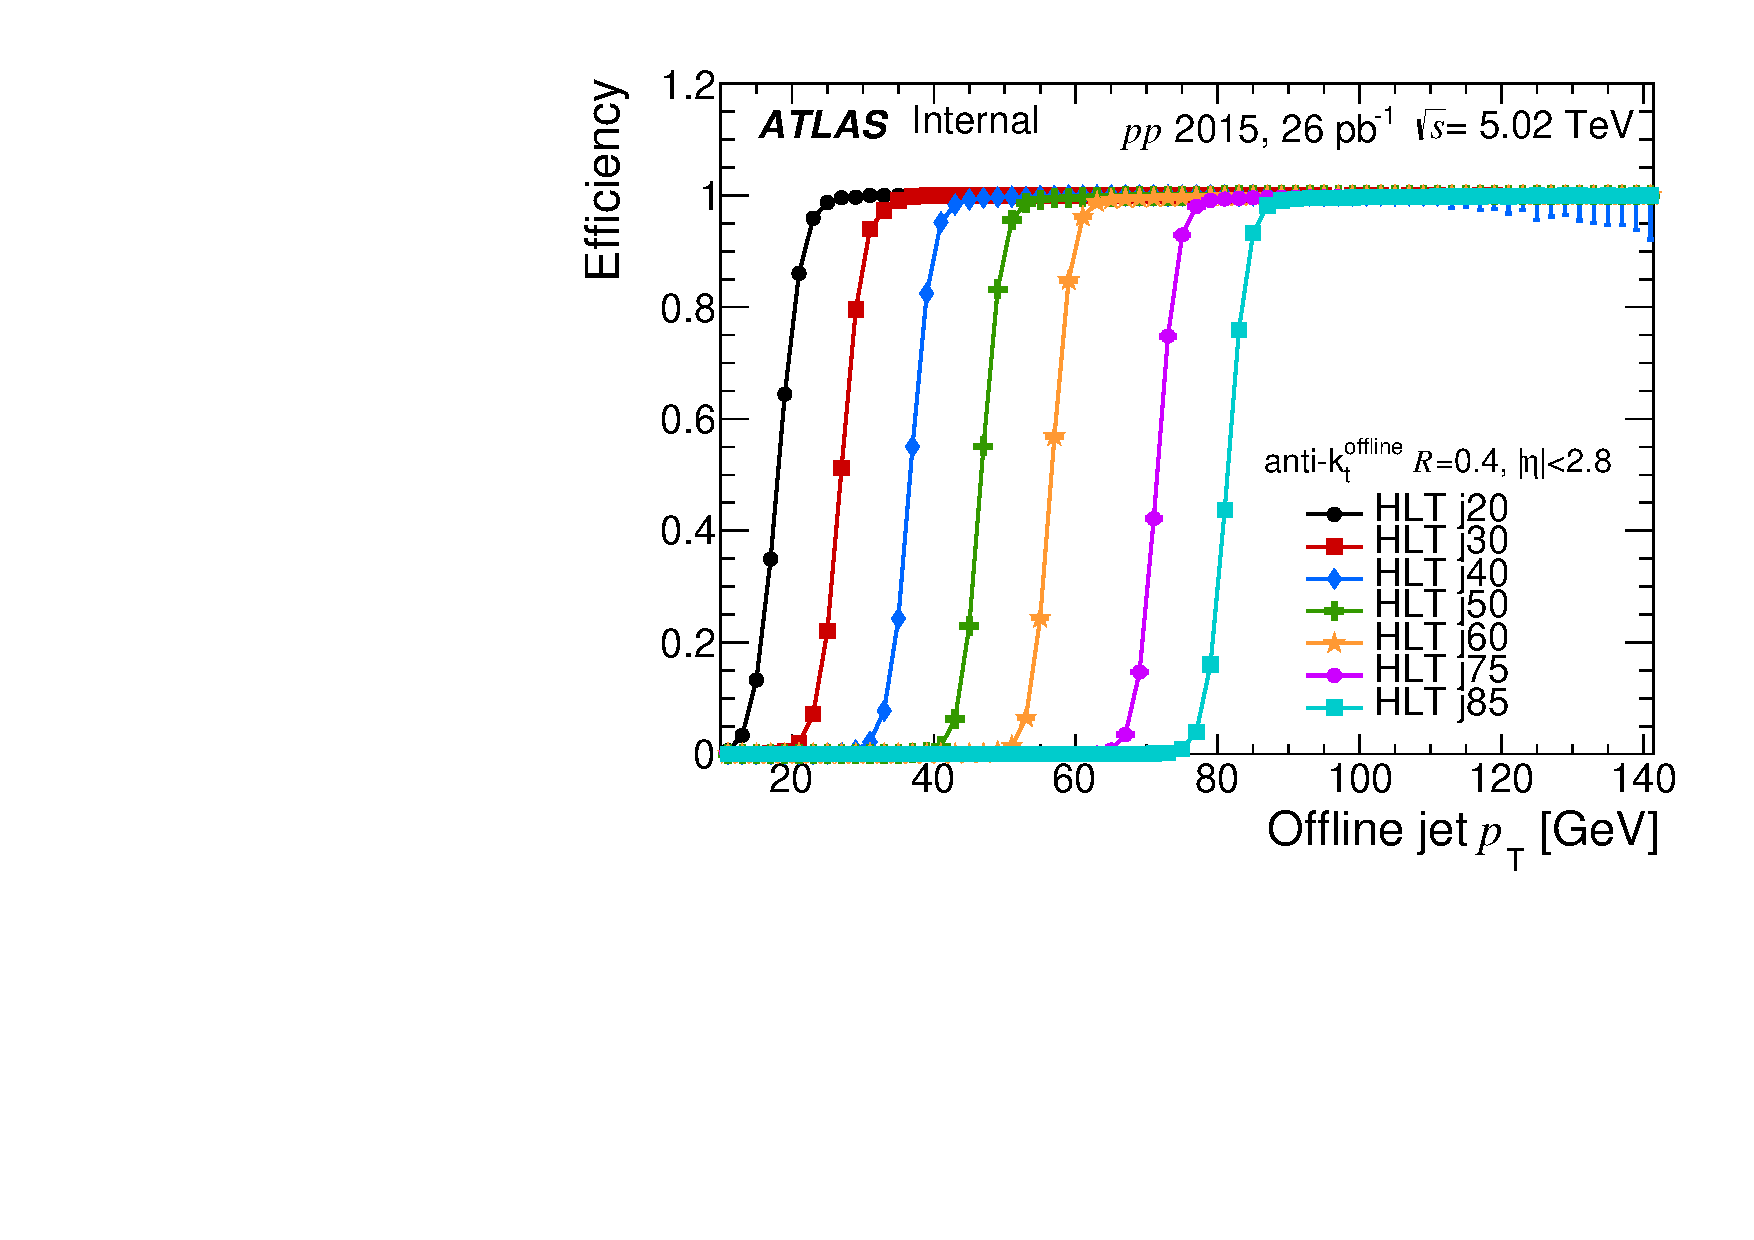
\includegraphics[width=0.75\textwidth]{figures_general/Eff_pp_5TeV_central.pdf}
}
 \caption{Trigger efficiencies for R=0.4 offline jets for seven HLT jet triggers in \pp\ collisions at 5.02 TeV.}
 \label{Fig:Trigger_pp5}
 \end{figure}


 \begin{figure}[h]
    \centerline{
       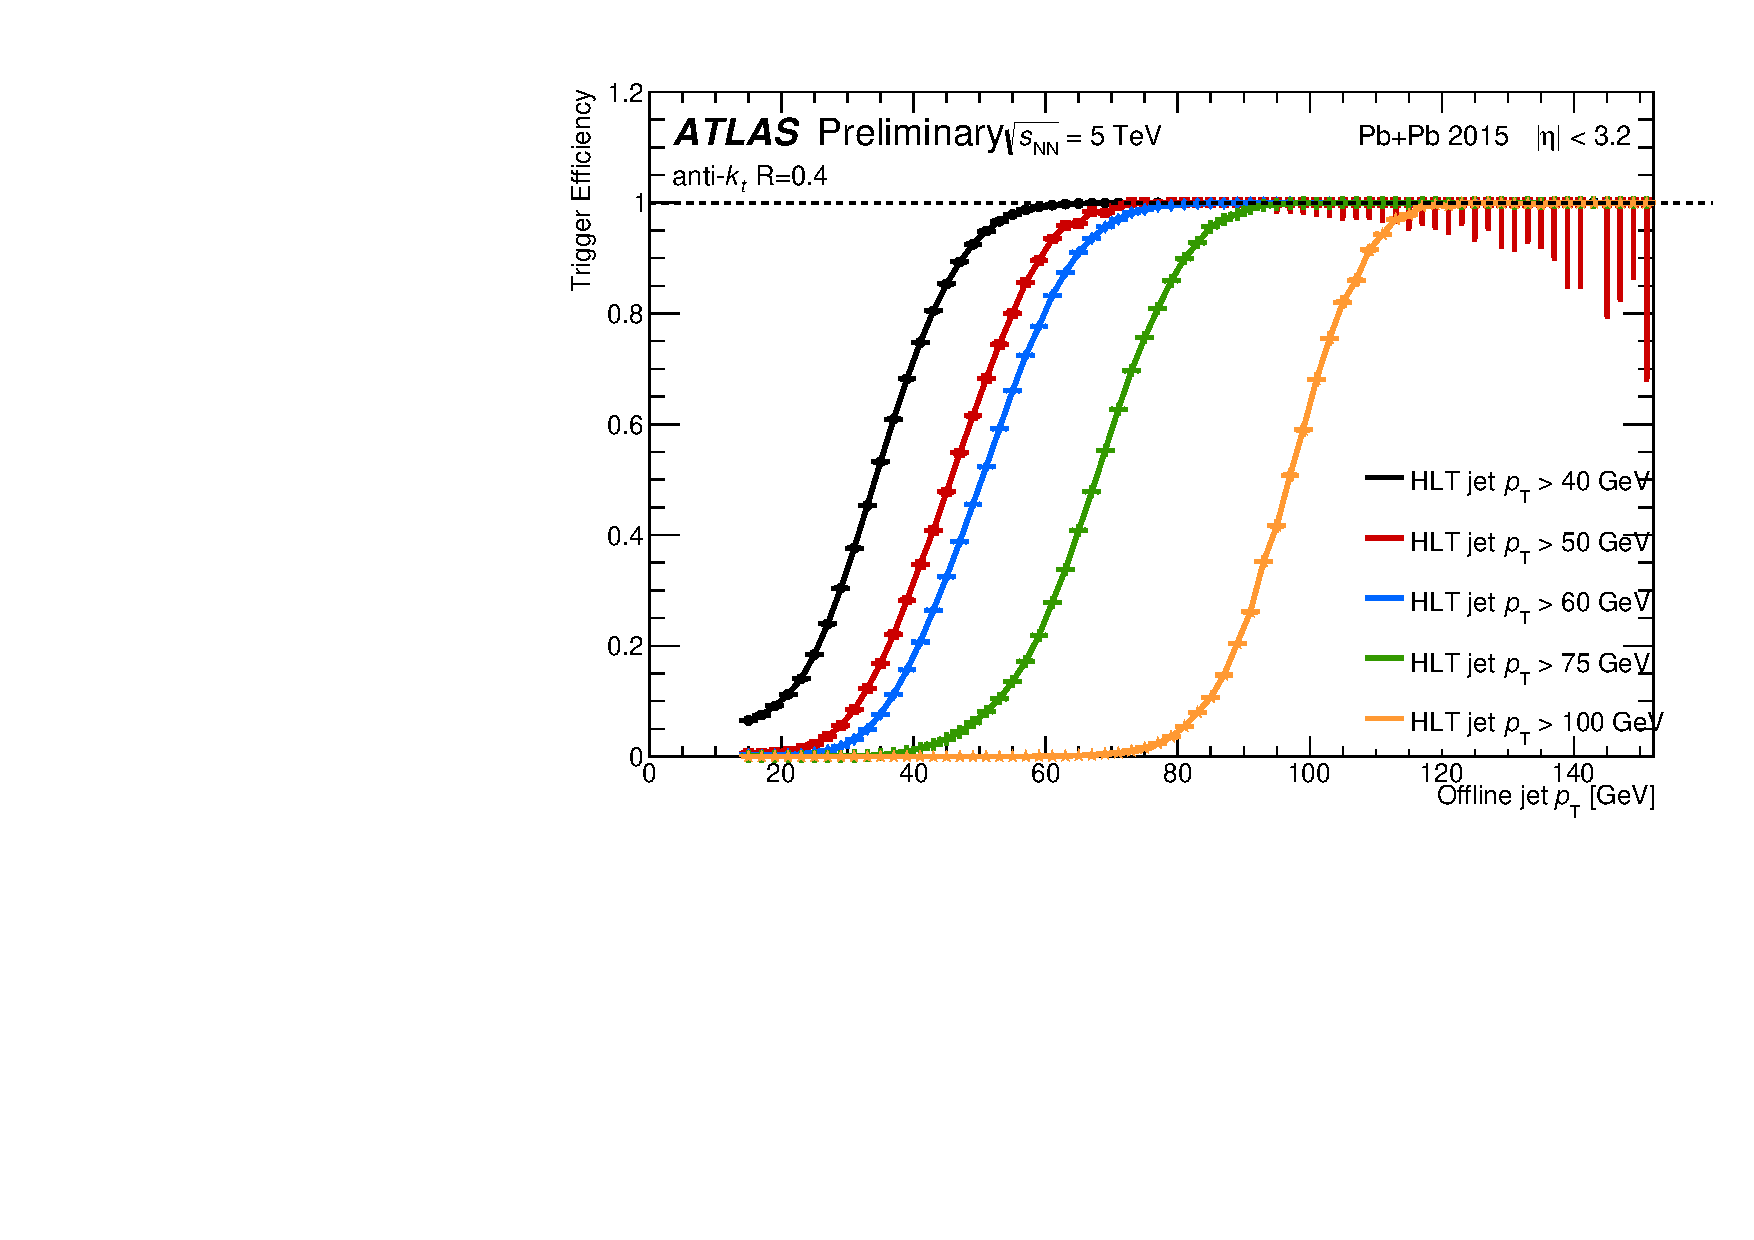
\includegraphics[width=0.75\textwidth]{figures_general/trigger_eff_PbPb_CentInclusive.pdf}
    }
    \caption{Jet trigger efficiency in centrality inclusive (0-80\%) \pbpb\ collisions for R=0.4 offline
    jets.}
    \label{fig:Trigger_PbPb}
 \end{figure}

In addition to the jet triggered sample, a MB triggered sample defined by a logical OR of the total energy trigger with a threshold of 50~\GeV\ and the ZDC coincidence trigger was used as part of the MC overlay procedure

The event fraction as a function of run number for both the hard probes stream and the minimum bias overlay stream in \pbpb\ is shown in Fig.~\ref{fig:evnt_fraction}

 \begin{figure}[h]
    \centerline{
       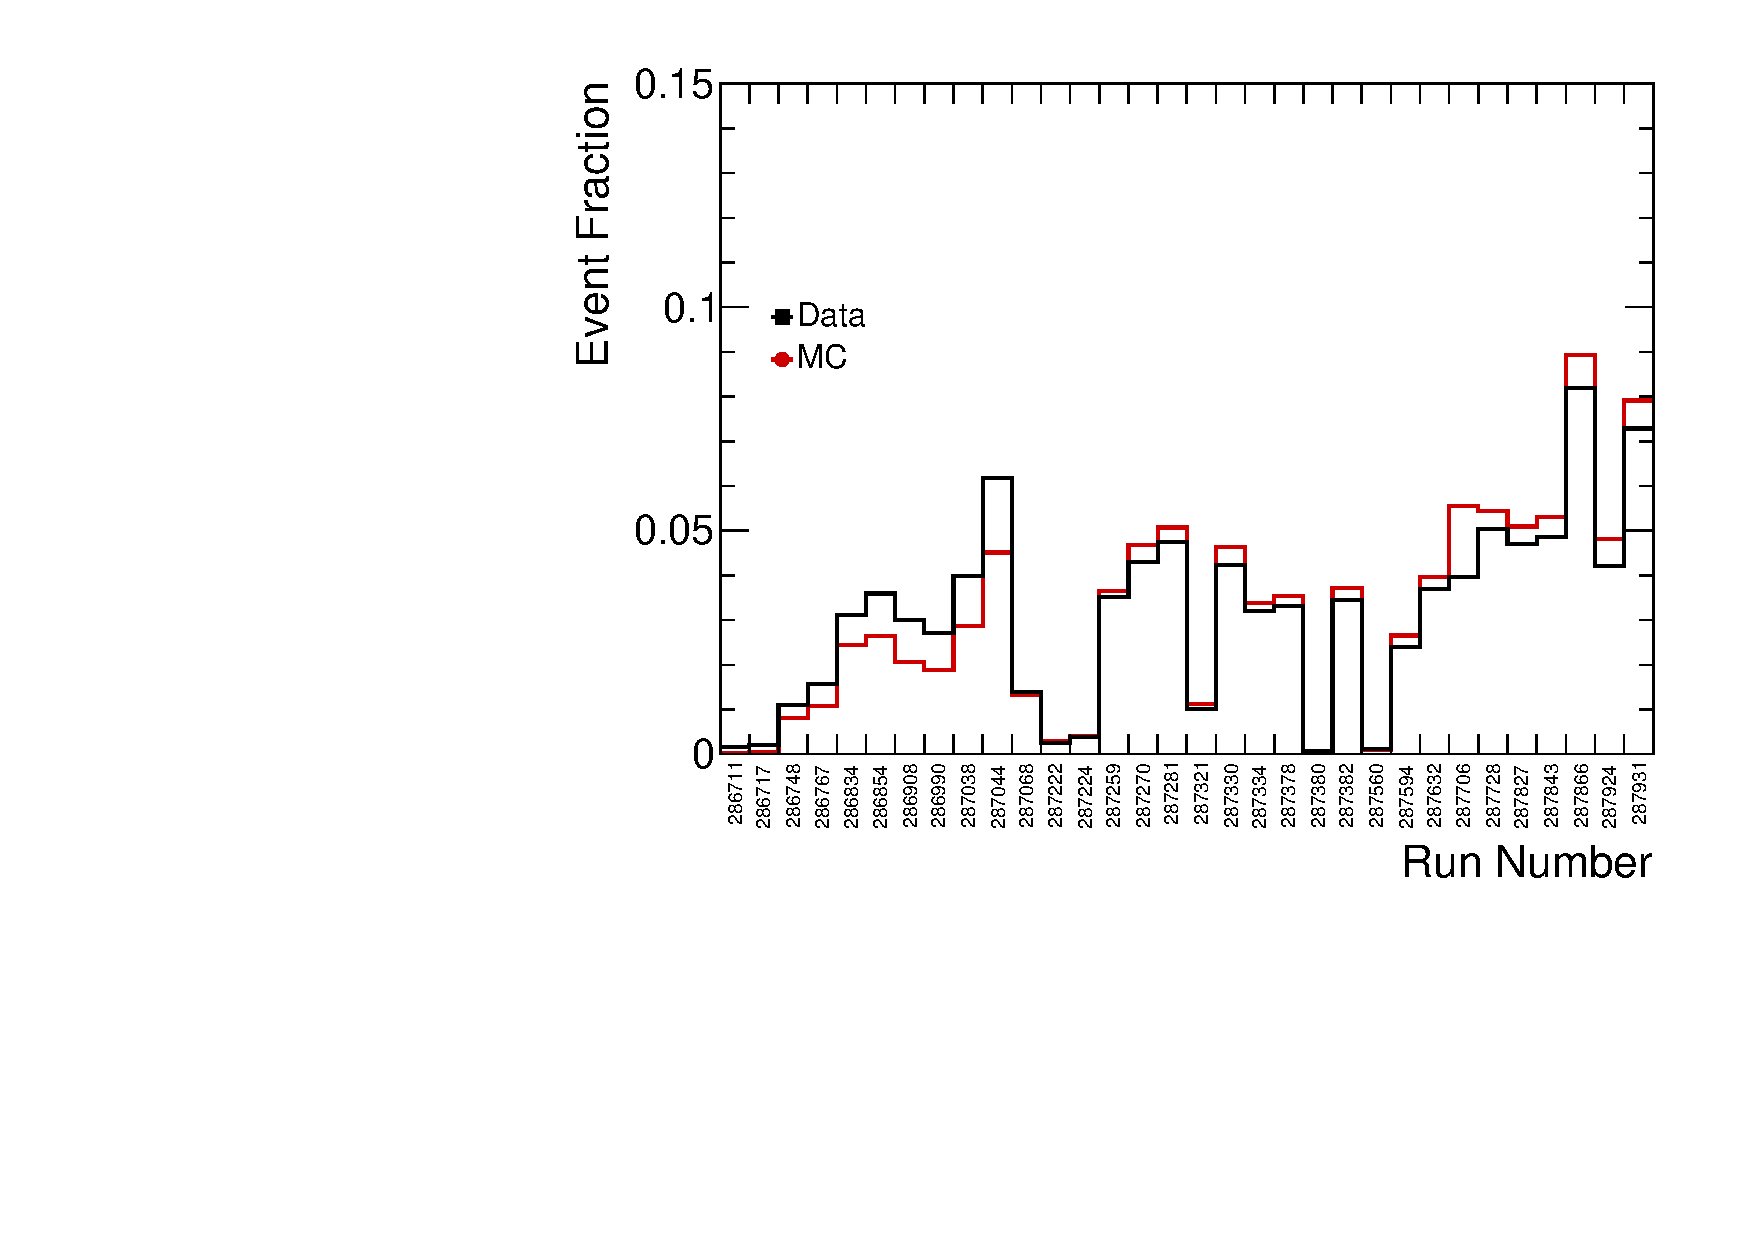
\includegraphics[width=0.9\textwidth]{figures_general/EventPercentages.pdf}
    }
    \caption{Event fraction as a function of runs for Hard Probes and the Minimum Bias Overlay Streams in \pbpb\ collisions.}
    \label{fig:evnt_fraction}
 \end{figure}

The run dependence of the underlying event (a core part of this measurement) was tested by dividing the data and MC into three periods with approximately equal number of events in each period: 286711 -- 287259, 287270 -- 287632, and 287706 -- 287931. The underlying event determined for each period compared to the nominal underlying event evaluated for the entire dataset is shown in Fig.\ref{fig:weighted_runs}, and it can be seen that the UE is stable throughout the data taking period.
%The systematic uncertainty associated with the run dependence was included in the calculation of the systematic uncertainty on the result.

 \begin{figure}[h]
    \centerline{
       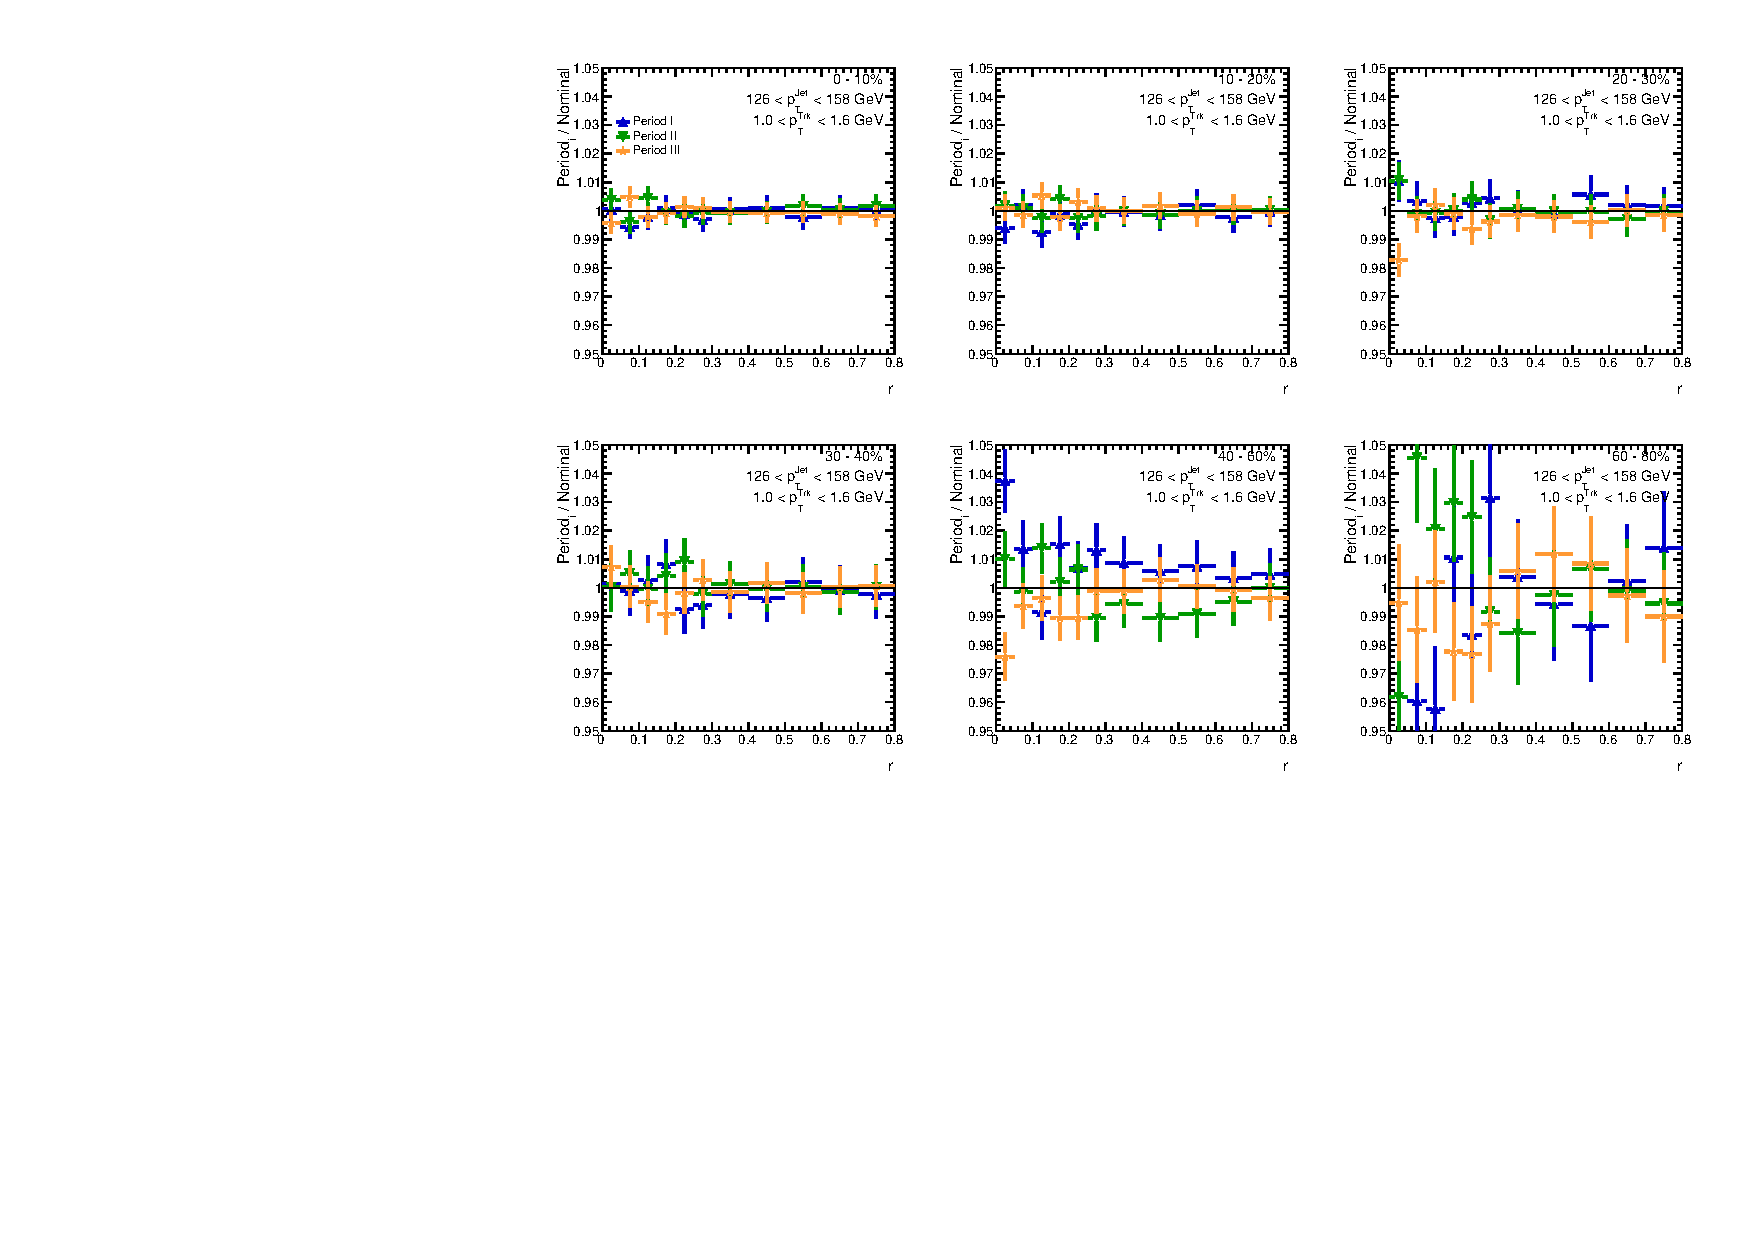
\includegraphics[width=0.75\textwidth]{figures_general/weightedRuns.pdf}
    }
    \caption{Stability of the underlying event for three different periods of the data taking. The different curves indicate the ratio of the underlying event in each period of data taking to the underlying event determined in the entire dataset.}
    \label{fig:weighted_runs}
 \end{figure}



% two separate MB data sample are used: 1) to estimate the underlying event contribution of charged particles to measured distributions; 2) to study detector performance in conditions that match the data. The first sample was recorded by MB triggers requiring either to have the transverse energy in the whole calorimeter exceeding 50 GeV at the Level-1 trigger (HLT\_noalg\_mb\_L1TE50) or to have a track reconstructed in the inner detector in coincidence with ZDC signals on both sides (HLT\_mb\_sptrk\_ion\_L1ZDC\_A\_C\_VTE50). The second sample was recorded with the MB trigger defined by a logical OR of the total energy trigger with a threshold of 50~\GeV\ and the ZDC coincidence trigger. This sample was used because it was utilized in the MC overlay procedure. Furthermore, two total transverse-energy triggers requiring 1.5~\TeV\ and 6.5~\TeV\ were used to enhance higher multiplicity events.

%
%   \begin{table}[h]
%\centering
%\begin{tabular}{|c|c|}
%\hline
%trigger & \ptjet (GeV) \\
%\hline
%%{\tt \footnotesize EF\_j20} & 25.7-35.2\\
%%{\tt \footnotesize EF\_j30\_L1TE5} & 35.2-43.6\\
%%{\tt \footnotesize EF\_j40\_L1TE5}  & 43.6-52.8\\
%%{\tt \footnotesize EF\_j50\_L1J12} & 52.8-62.5\\
%%{\tt \footnotesize EF\_j60\_L1J15} & 62.5-78.8\\
%%{\tt \footnotesize EF\_j75\_L1J20} & 78.8-88.8\\
%{\tt \footnotesize EF\_j85} & $>$~88.8\\
%\hline
%\end{tabular}
%\caption{Triggers used in the analysis of 2015 \pp\ data and the corresponding \ptjet\ ranges.}
%\label{tab:jettrigpp5}
%\end{table}
%
%\begin{table}
%\centering
%\begin{tabular}{|c|c|}
%\hline
%trigger & \ptjet (GeV) \\
%\hline
%{\tt \footnotesize EF\_j75\_ion\_L1TE50} & $>$~91\\
%%{\tt \footnotesize EF\_j100\_ion\_LITE50} & $>$~114\\
%\hline
%\end{tabular}
%\caption{Triggers used in the analysis of 2015 \pbpb\ data and the corresponding \ptjet\ ranges.}
%\label{tab:jettrigpbpb5}
%\end{table}


\subsection{Monte Carlo Samples}
%The studies in this note utilize high-statistic MC samples that are used to study the performance of the analyses and in the unfolding procedure. The MC12 PYTHIA6.4 \pp\ di-jet events at $\sqrt{s} =5.02$~TeV with the same rapidity shift in the center of mass as in the data, were embedded on top of heavy ion MB data events collected during the 2013 run using a MB trigger in \texttt{MinBiasOverlay} stream. The \texttt{MinBiasOverlay} records the data without zero suppression. The signal from this trigger was combined with the signal from PYTHIA6.4 at the digitization stage and then reconstructed as a combined event. MC samples are used for both the period A and period B running conditions. Truth jets with \pTtrue\ were defined in the MC sample as the output of the \antikt\ algorithm with \RFour\ applied to the final-state particles generated by PYTHIA6.4.

 

This analysis also utilizes MC15 \pythiaeight\ \pp\ jet events at $\sqrt{s} =5.02$~TeV with the A14 ATLAS tune and the NNPDF23LO pdfs~\cite{ATL-PHYS-PUB-2014-021}. The definitions of the \pp\ MC samples can be found in Tab.~\ref{Tab:MCSamples_pp5}. The \pbpb\ MC uses POWHEG+\pythiaeight\ events that are overlayed on top of MB \PbPb\ collisions.  
These samples are listed in Tab.~\ref{tab:overlay}. 

\begin{table}[htbp]
\centering
\begin{tabular}{|l|p{0.65\linewidth}|}
\hline
\multicolumn{1}{|c|}{JZ} & \multicolumn{1}{c|}{Dataset Name}                 		                                  \tabularnewline \hline
2	& {\tt \footnotesize mc15\_5TeV.420022.PowhegPythia8EvtGen\_A14\_NNPDF23LO\_CT10ME\_ jetjet\_JZ2R04.merge.DAOD\_HION7.e4109\_s2860\_r7792\_r7676\_p3442}                                                     \tabularnewline \hline
3	& {\tt \footnotesize mc15\_5TeV.420023.PowhegPythia8EvtGen\_A14\_NNPDF23LO\_CT10ME\_ jetjet\_JZ3R04.merge.DAOD\_HION7.e5067\_s2860\_r7792\_r7676\_p3442}                                                                                  \tabularnewline \hline
4	& {\tt \footnotesize mc15\_5TeV.420024.PowhegPythia8EvtGen\_A14\_NNPDF23LO\_CT10ME\_ jetjet\_JZ4R04.merge.DAOD\_HION7.e5067\_s2860\_r7792\_r7676\_p3442}                                                                   \tabularnewline \hline
\end{tabular}
\begin{tabular}{| c | c | c | c | c |} \hline
J & \RFour\ \pTtrue\ [\GeV]  & $\sigma$ [$\mathrm{nb}$] $\times$ $\epsilon$ & $\#$events \\ \hline
2  & 60--160 &  (6.4 $\times$ 10$^5$) $\times$ (4.27 $\times$ 10$^{-3}$) & 5.8 M \\ \hline
3  & 160--400 &  (4.7 $\times$ 10$^3$) $\times$ (5.28 $\times$ 10$^{-3}$) & 5.9 M \\ \hline
4  & 400--800 &  (2.7 $\times$ 10$^1$)  $\times$ (4.58 $\times$ 10$^{-3}$) & 5.8 M \\ \hline
\end{tabular}
\caption{5.02 TeV \pythiaeight\ \pp\ MC samples.}
\label{Tab:MCSamples_pp5}
\end{table}


\begin{table}[htbp]
\centering
\begin{tabular}{|l|p{0.65\linewidth}|}
\hline
\multicolumn{1}{|c|}{JZ} & \multicolumn{1}{c|}{Dataset Name}                 		                                  \tabularnewline \hline
2	& {\tt \footnotesize mc15\_5TeV.420022.PowhegPythia8EvtGen\_A14\_NNPDF23LO\_CT10ME\_jetjet \_JZ2R04.merge.DAOD\_HION7.e4109\_d1421\_r8238\_r8052\_p3196}                                                     \tabularnewline \hline
3	& {\tt \footnotesize mc15\_5TeV.420023.PowhegPythia8EvtGen\_A14\_NNPDF23LO\_CT10ME\_jetjet \_JZ3R04.merge.DAOD\_HION7.e4109\_d1421\_r8238\_r8052\_p3196}                                                                                  \tabularnewline \hline
4	& {\tt \footnotesize mc15\_5TeV.420024.PowhegPythia8EvtGen\_A14\_NNPDF23LO\_CT10ME\_jetjet \_JZ4R04.merge.DAOD\_HION7.e4109\_d1421\_r8238\_r8052\_p3196}                                                                   \tabularnewline \hline
\end{tabular}
\caption{\pbpb\ data overlay datasets used here.}
\label{tab:overlay}
\end{table}

\clearpage
